\hypertarget{part-1-design-3}{%
\section{Part 1, design 3}\label{part-1-design-3}}

\centering
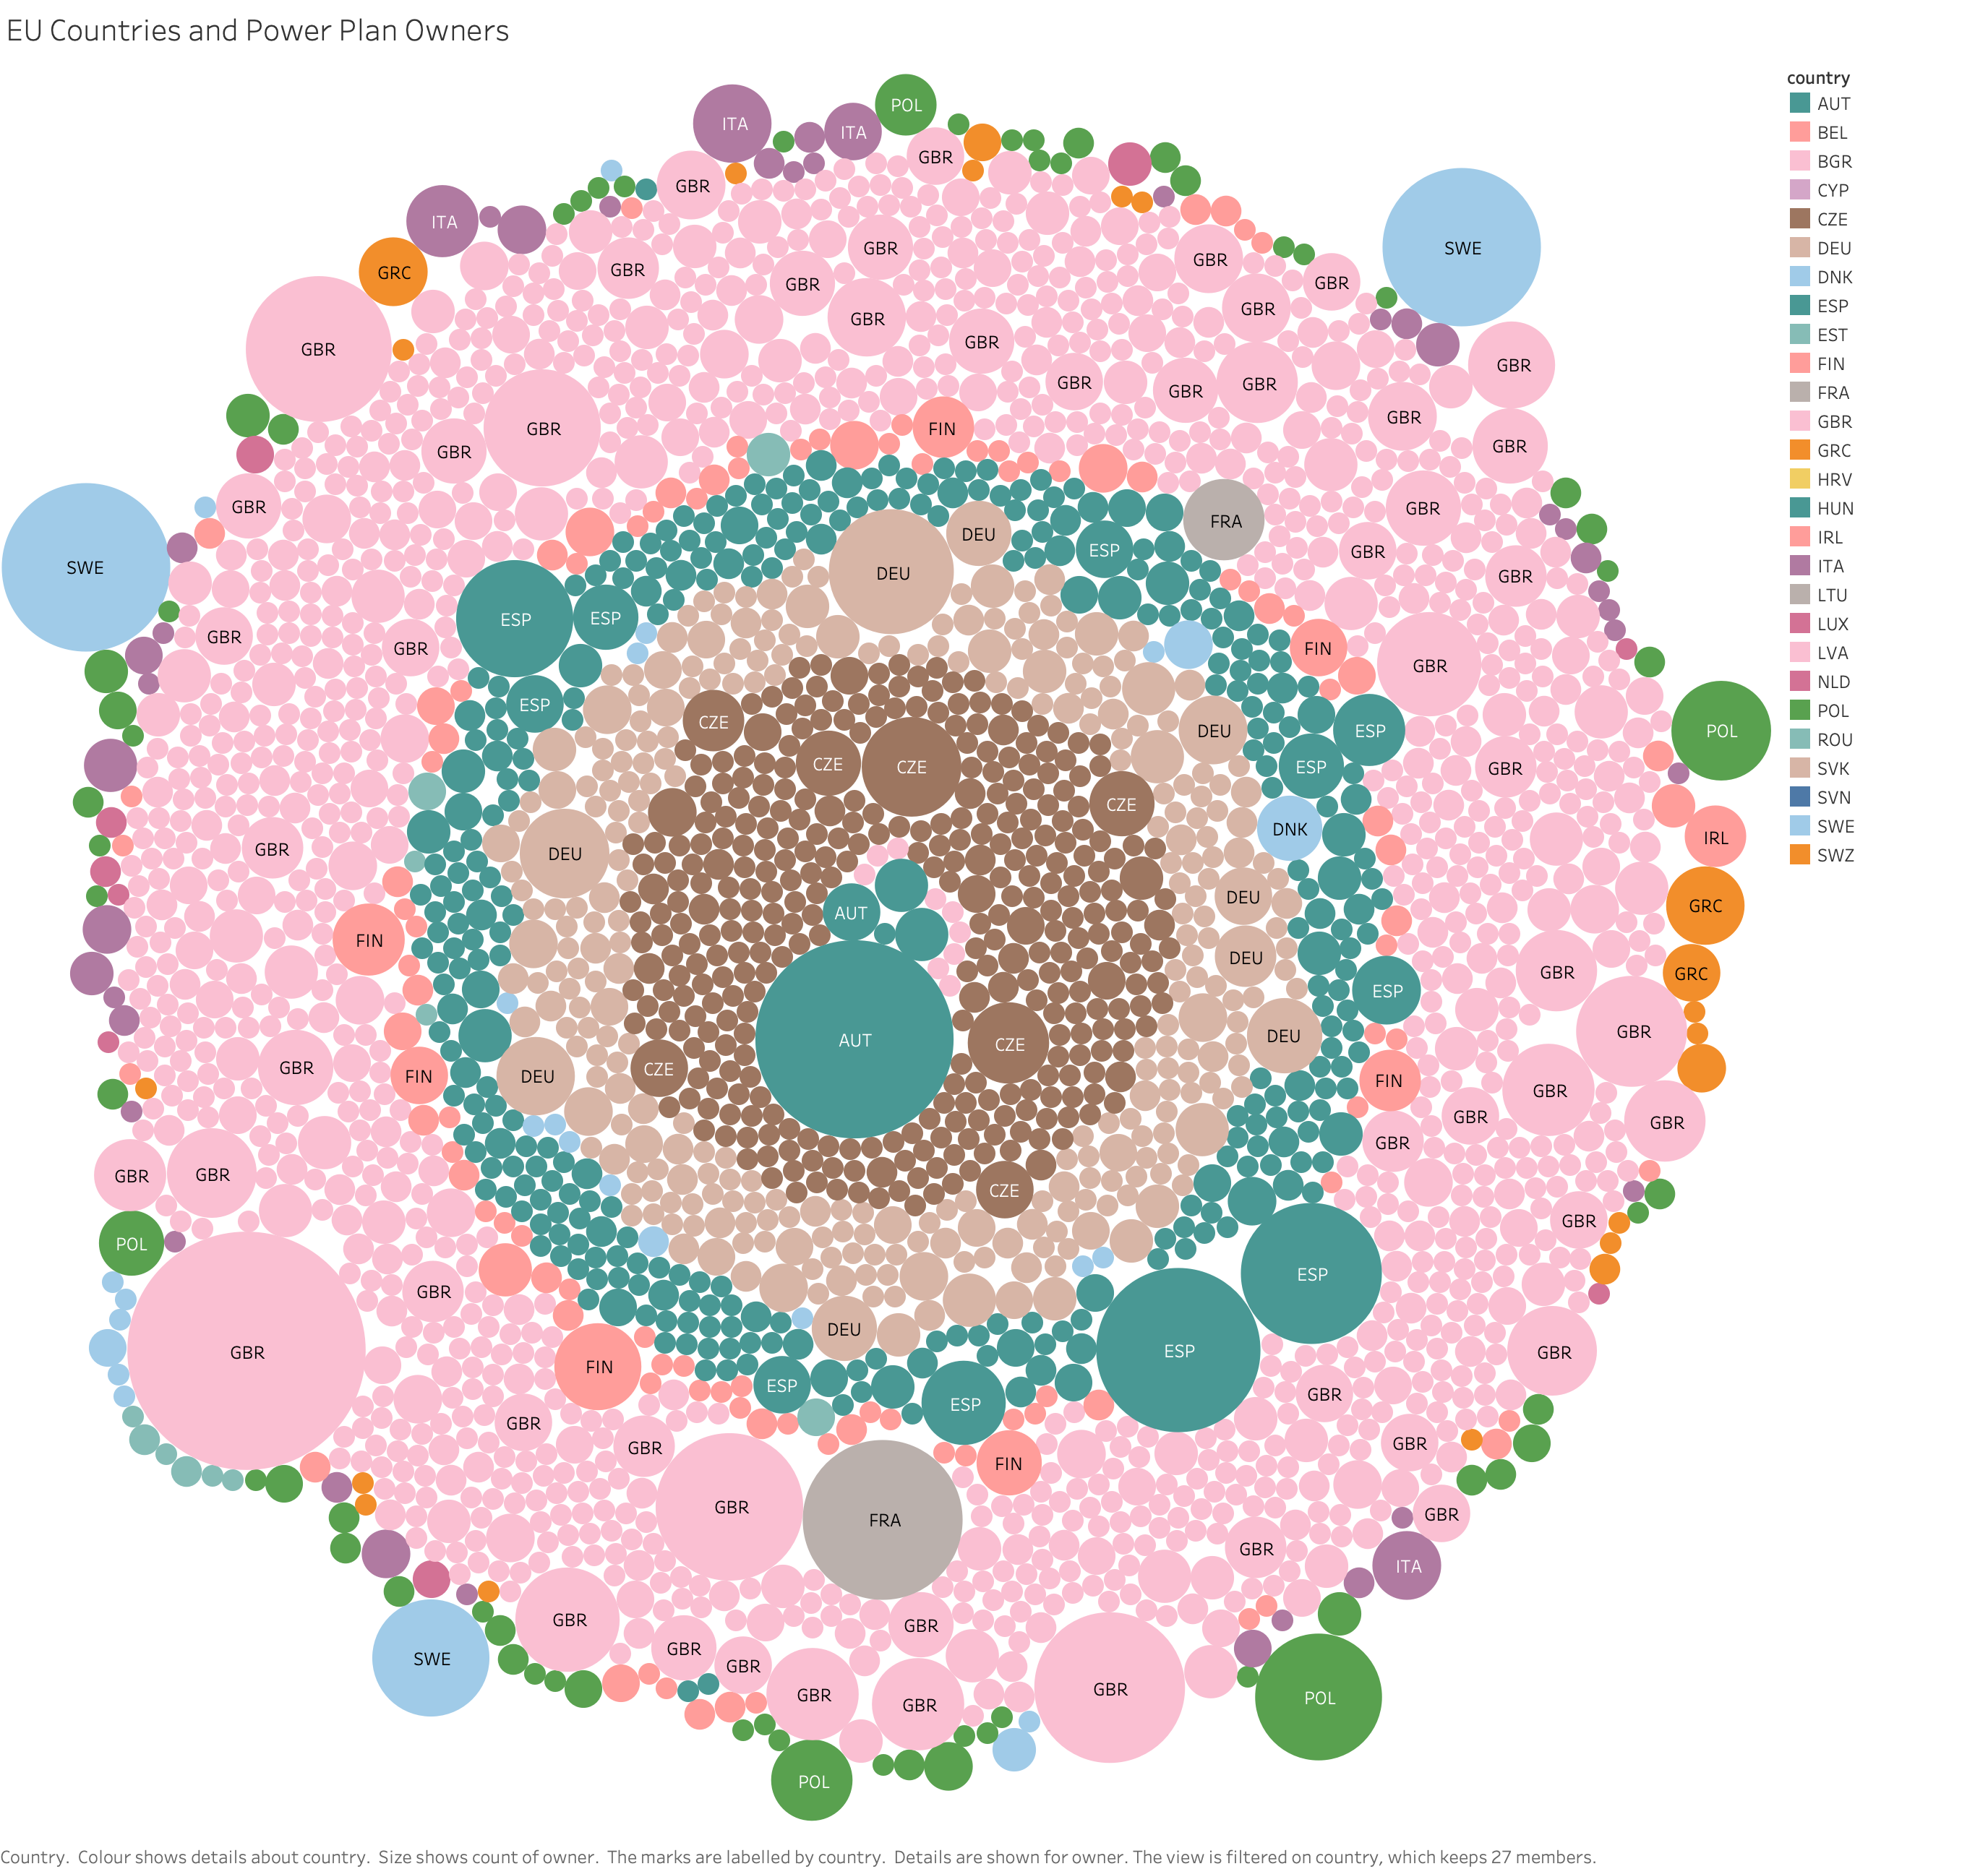
\includegraphics[height=10cm]{Viz3.png}

\hypertarget{description}{%
\subsubsection{Description}\label{description}}

\begin{description}
\item[Visual Design Type:]
Packed Bubbles
\item[Name of Tool:]
Tableau
\item[Country:]
EU members including the UK.  Austria, Belgium, Bulgaria, Cyprus, Czech Republic, Germany, Denmark, Estonia, Spain, Finland, France, United Kingdom, Greece, Croatia, Hungary, Ireland, Italy, Lithuania, Luxembourg, Latvia, Malta, Netherlands, Poland, Portugal, Romania, Sweden, Slovenia, Slovakia.
\item[Year:]
1896 - 2018
\item[Visual Mappings:]
\begin{itemize}
	\tightlist
	\item[  ]
\end{itemize}
\begin{itemize}
\tightlist
\item
  \textbf{mapping 1}: The count of the owner was used to generate the size of the bubbles. 
\end{itemize}

\begin{itemize}
\tightlist
\item
  \textbf{mapping 2}: The owner was also used as a detail as well as the sum of the number of records on the visualisation. Country was used for the colour coding and also used for the tooltip.
\end{itemize}
\item[Unique Observation:]
All of France’s power plants are owned by two companies, EDF and GDF-Suez. While the Great Britton has the most amount of different owners for their power plants.
\item[Data Preparation:]
Data was filtered by country.
\end{description}